\documentclass[11pt]{article}
 
\usepackage[margin=.95in]{geometry} 
\usepackage{amsmath,amsthm,amssymb, graphicx, multicol, array}
 
\newcommand{\N}{\mathbb{N}}
\newcommand{\Z}{\mathbb{Z}}
 

\begin{document}
 
\title{Homework 5}
\author{Juliette Franqueville\\
}
\maketitle

\subsection*{(1) (a)}


\begin{figure}[!h]
    \centering
    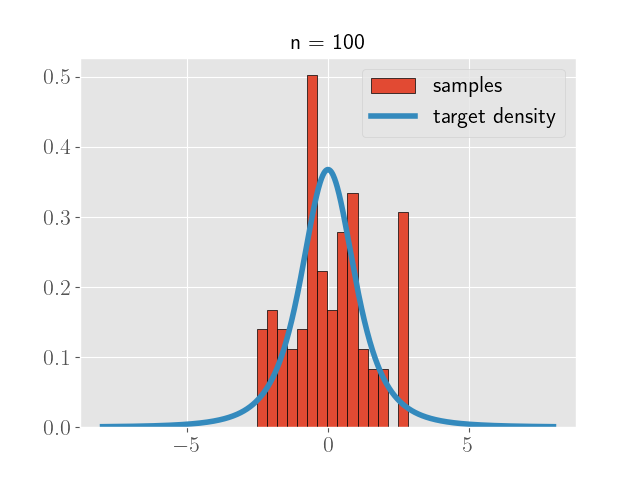
\includegraphics[scale=.5
    ]{../figures/resamples_n_100.png}
    \caption{samples and t distribution for $n=100$}
    \label{fig:my_label}
\end{figure}

\begin{figure}[!h]
    \centering
    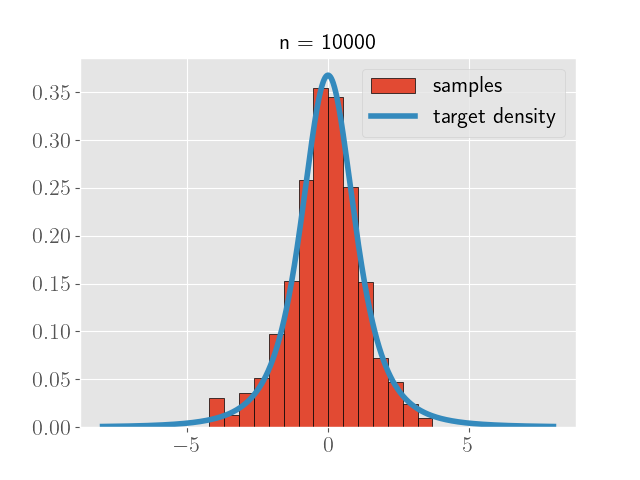
\includegraphics[scale=.5
    ]{../figures/resamples_n_10000.png}
    \caption{samples and t distribution for $n=10,000$}
    \label{fig:my_label}
\end{figure}
\newpage

\subsection*{(b)}
For $n=100$, the estimated mean and variance were 0.12 and 0.84, respectively. For $n=10,000$, they were 0.03 and 1.67. The means were close to the actual mean (0), but the variances were underestimated compared to the actual variance of $t_3$ (3). This is not suprising because the tails of the normal are not as wide as those of the $t$ distribution. In other words, the normal distribution does not fully cover the $t$ distribution, so the points far from the mean in the tails do not get sampled, which makes the variance too small. I redid this exercise with a uniform distribution that  covered $t_3$ better, and the variances were closer to 3.

\subsection*{(2)}
\begin{align*}
    (X_1|X_2) & \propto (X_1, X_2)\\
    & \propto (1-\rho^2)^{-1/2}\text{exp} \left( -\frac{1}{2(1-\rho^2)} \begin{bmatrix} x_1-\mu_1, &x_2-\mu_2 \end{bmatrix} \begin{bmatrix} 1 & -\rho \\ -\rho & 1 \end{bmatrix}\begin{bmatrix} x_1-\mu_1 \\ x_2-\mu_2 \end{bmatrix}\right)\\
    & \propto (1-\rho^2)^{-1/2}\text{exp} \left( -\frac{1}{2(1-\rho^2)}[(x_1-\mu_1)^2-2\rho(x_1-\mu_1)(x_2-\mu_2) + (x_2-\mu_2)^2] \right)\\
     & \propto (1-\rho^2)^{-1/2}\text{exp} \left( -\frac{1}{2(1-\rho^2)}[x_1^2-2x_1(\mu_1+\rho x_2 - \rho x_1)] \right)\\
     & \propto \mathcal{N}(\mu_1 + \rho(x_2-x_1), 1-\rho^2)
\end{align*}

To get $(X_2|X_1)$, we simply swap $X_1$ ad $X_2$. We then use a Gibbs sampler to produce the following plots. I set burn in $=500$ and thin every 2 iterations.


\end{document}
